\documentclass[11pt,letterpaper]{article}
\usepackage[lmargin=1in,rmargin=1in,tmargin=1in,bmargin=1in]{geometry}
\usepackage{../style/homework}
\usepackage{../style/commands}
\setbool{quotetype}{false} % True: Side; False: Under
\setbool{hideans}{true} % Student: True; Instructor: False

% -------------------
% Content
% -------------------
\begin{document}

\homework{5: Due 10/06}{Martini. Gin, not vodka. Obviously. Stirred for 10~seconds while glancing at an unopened bottle of vermouth.}{Gary `Eggsy' Unwin, The Kingsman}


% Problem 1
\problem{10} Plot the function $f(x):= 3 - 2x$, being as accurate as possible. 
	\[
	\fbox{
	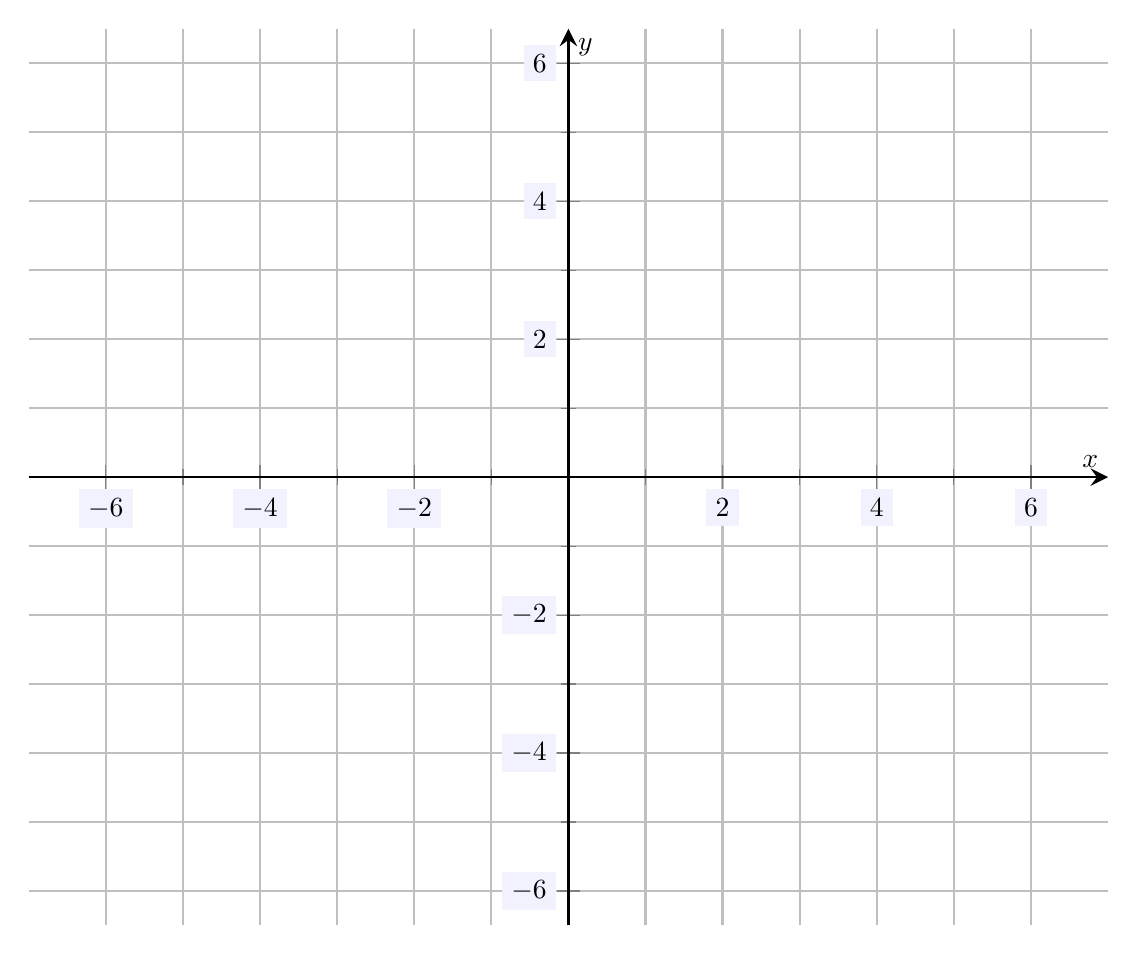
\begin{tikzpicture}[scale=2,every node/.style={scale=0.5}]
	\begin{axis}[
	grid=both,
	axis lines=middle,
	ticklabel style={fill=blue!5!white},
	xmin= -7, xmax=7,
	ymin= -6.5, ymax=6.5,
	xtick={-6,-4,-2,0,2,4,6},
	ytick={-6,-4,-2,0,2,4,6},
	minor tick = {-5,-3,...,5},
	xlabel=\(x\),ylabel=\(y\),
%	samples=20
	]
%	\addplot[thick, domain= -7:-3] {-3*x-10};
%	\addplot[thick,domain= -3:2] {4/5*x-3/5};
%	\addplot[thick,domain= 2:4] {7/2*x^2-41/2*x+28};
%	\addplot[thick,domain= 4:7] {2};
%	\addplot[holdot] coordinates{(-3,-1)(2,1)(4,2)};
%	\addplot[soldot] coordinates{(-3,-3)(4,3)};
	\end{axis}
	\end{tikzpicture}
	}
	\]





\newpage





% Problem 2
\problem{10} Plot the function $f(x):= x^2 + 2x - 3$, being as accurate as possible. 
	\[
	\fbox{
	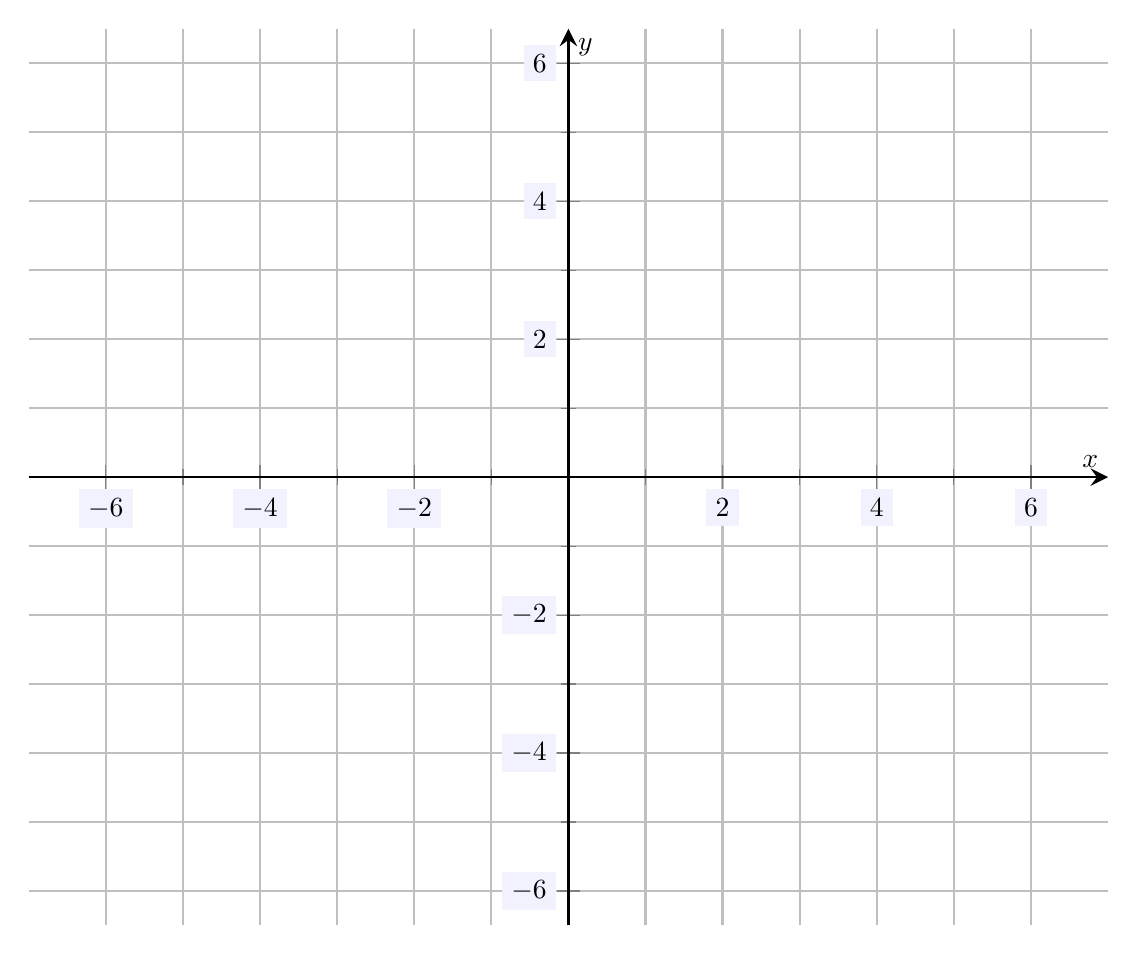
\begin{tikzpicture}[scale=2,every node/.style={scale=0.5}]
	\begin{axis}[
	grid=both,
	axis lines=middle,
	ticklabel style={fill=blue!5!white},
	xmin= -7, xmax=7,
	ymin= -6.5, ymax=6.5,
	xtick={-6,-4,-2,0,2,4,6},
	ytick={-6,-4,-2,0,2,4,6},
	minor tick = {-5,-3,...,5},
	xlabel=\(x\),ylabel=\(y\),
	]
	\end{axis}
	\end{tikzpicture}
	}
	\]





% Problem 3
\problem{10} Plot the function $f(x):= \dfrac{x - 1}{x^2 + 1}$, being as accurate as possible. 
	\[
	\fbox{
	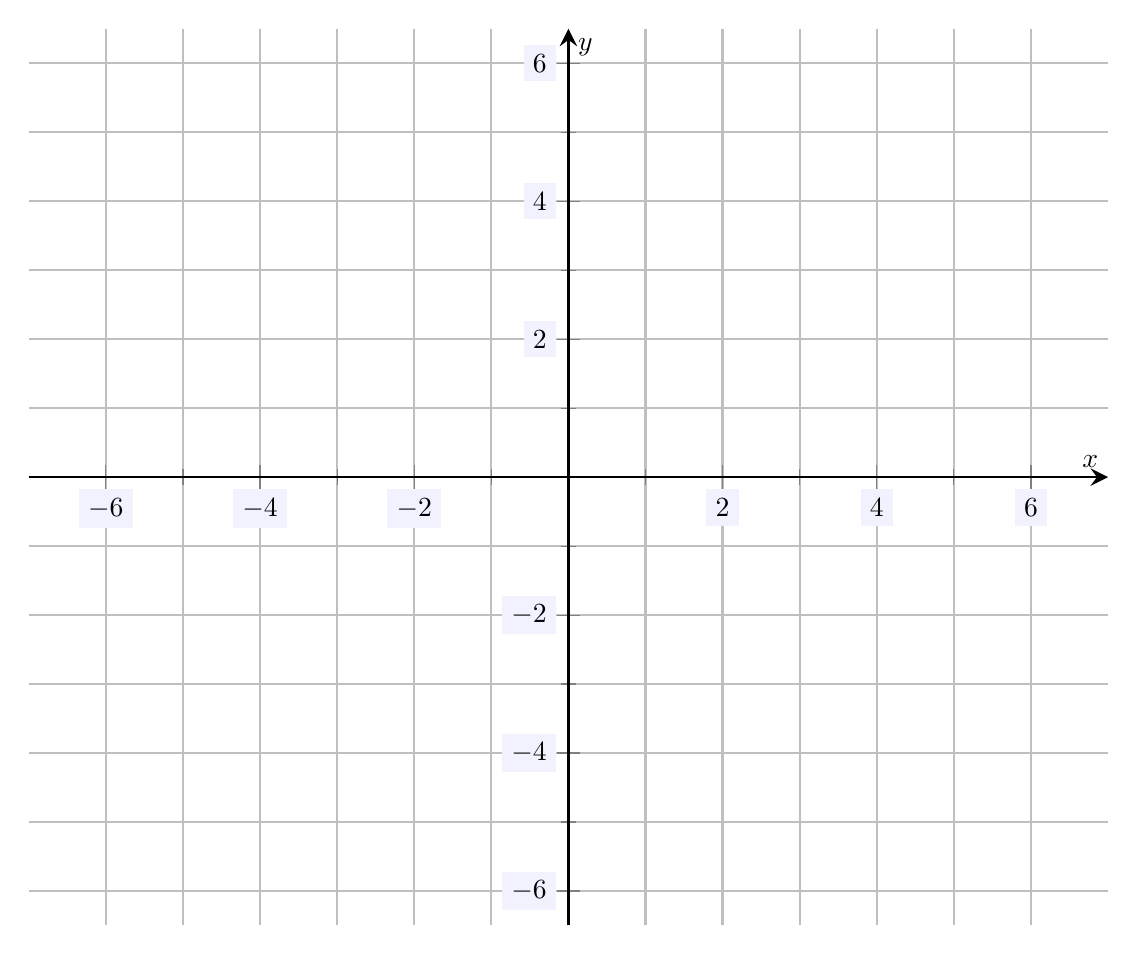
\begin{tikzpicture}[scale=2,every node/.style={scale=0.5}]
	\begin{axis}[
	grid=both,
	axis lines=middle,
	ticklabel style={fill=blue!5!white},
	xmin= -7, xmax=7,
	ymin= -6.5, ymax=6.5,
	xtick={-6,-4,-2,0,2,4,6},
	ytick={-6,-4,-2,0,2,4,6},
	minor tick = {-5,-3,...,5},
	xlabel=\(x\),ylabel=\(y\),
	]
	\end{axis}
	\end{tikzpicture}
	}
	\]





\newpage





% Problem 4
\problem{10} Let $f(x):= 4x - 7$.
	\begin{enumerate}[(a)]
	\item Find $f(1)$. \vfill
	\item What value(s) for $x$ make the output of $f(x)$ twice the output from (a)? \vfill
	\item Is $(1, 1)$ on the graph of $f(x)$? Explain. \vfill
	\item Is $(3, 5)$ on the graph of $f(x)$? Explain. \vfill
	\end{enumerate}





\newpage





% Problem 5
\problem{10} Define the following functions:
	\[
	\begin{aligned}
	f(x)&:= x - x^3 \\
	g(x)&:= x^2 - 3x + 1 \\
	h(x)&:= x^4 + 1
	\end{aligned}
	\]
Determine if the functions $f(x)$, $g(x)$ and $h(x)$ are even functions, odd functions, or neither. Be sure to justify your answer. 





\newpage





% Problem 6
\problem{10} Consider the function $f(x)$ plotted below. 
	\[
	\fbox{
	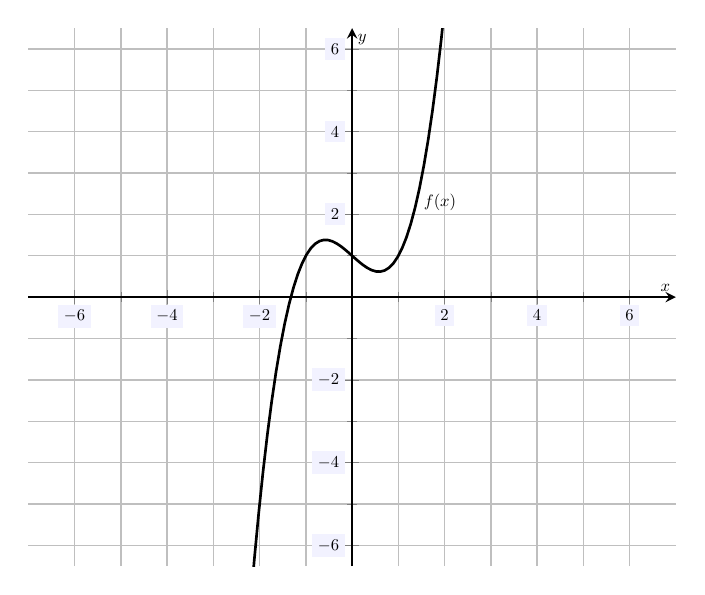
\begin{tikzpicture}[scale=1.2,every node/.style={scale=0.5}]
	\begin{axis}[
	grid=both,
	axis lines=middle,
	ticklabel style={fill=blue!5!white},
	xmin= -7, xmax=7,
	ymin= -6.5, ymax=6.5,
	xtick={-6,-4,-2,0,2,4,6},
	ytick={-6,-4,-2,0,2,4,6},
	minor tick = {-5,-3,...,5},
	xlabel=\(x\),ylabel=\(y\),
	samples=150
	]
	\node at (1.9,2.3) {$f(x)$};
	\addplot[thick,domain= -7:7] {x^3 - x + 1};
	\end{axis}
	\end{tikzpicture}
	}
	\]

\begin{enumerate}[(a)]
\item What is $f(-1)$? \vfill
\item Is the point $(1,1)$ on the graph of $f(x)$? Explain. \vfill
\item Is the point $(-2,3)$ on the graph of $f(x)$? Explain. \vfill
\item Is the function $f(x)$ even, odd, or neither. Explain. \vfill
\end{enumerate}





%\printpoints
\end{document}